\chapter{Discussion}
%As shown in this thesis, micro-tasking is used in projects that wish to exploit human computation and a huge crowd, through for instance crowdsourcing. This thesis study if micro-tasking can or should expand to involve interactive maps and geospatial data. In OpenStreetMap, it has become a dominant method, both in mapping jobs and imports jobs \citep{Erichsen2016}. The methods popularity in OSM confirms the potential of expanding micro-tasking to the geo-community. The research questions tested is: 1) Is it possible to give micro-tasks containing geospatial data to inexperienced workers? 2) Will the quality of the solved task increase with fewer elements present in each micro-task? 3) What are the number of elements optimal within a micro-task to get it completed as quickly as possible?

Our results have found support for the possibility of giving geospatial micro-tasks to all individuals, independent of background. There was statistically significant evidence that inexperienced participants finished the tasks faster than experienced participants, this is also shown in figure \ref{fig:meanstdparticipantstime}. The mean time difference was 16 seconds, a statistically significant, but relatively small difference. One would expect that experienced participants finished the tasks faster since they are familiar with map interaction and interpreting base maps and meta information. During the pilot test, the author noticed that the experienced participants used the map aids given in question one more frequently than inexperienced. The map aids were zoom, panning and a layer control to show/hide the building footprints. A possible explanation for the time difference is that the experienced participants spent more time using the map aids provided since they are more familiar with them and knew how to use them. It is a possibility of them making the tasks more complicated than necessary. Experienced individuals have experience of solving much more complex tasks and maybe compares the micro-tasks with more advanced tasks, overestimating the complexity.

When analyzing the number of correctly chosen elements between experienced and inexperienced participants, the difference is not statistically significant. Figure \ref{fig:meanstdparticipantscorrect} show a very similar mean value in the number of correct elements. Inexperienced participants had a mean of 9.83 correct elements, while experienced had a mean of 9.81 correct elements. One would expect that inexperienced participants had fewer correct elements since they spent less time on the tasks. \cite{Salk2016} results also observed minor differences between the professional and non-professional participants. They concluded that professional background had a limited first-order relationship with task accuracy. It can be argued that the design of the question interfaces, together with the introduction video and training task, was so easy to use that the professional background had no effect on the quality of the task results. \cite{See2013} concluded that with proper targeted training material the differences between experts and non-experts can decrease. One can also suspect the experienced participants did not follow the instructions video as carefully as inexperienced since they already knew how to use interactive maps. This statement cannot be verified.

The splitting of participants into experienced and inexperienced was based on the question "Do you have experience of working with geospatial data?". Other studies ask the participants for background information through a registration procedure. \cite{See2013} and \cite{Salk2016} considered people with a background in remote sensing/spatial science as experts, and people who were new to the discipline or had a self-declared limited background as non-experts. In this study, the participants are self-declared experts / non-experts. It is not possible to validate this information. In the pilot-test we knew the background of the participants, they answered yes and no on the experience question as the author anticipated. 

There were minor differences between the three tasks. Results found no statistical support for faster completion time with fewer elements. The statistical analysis concluded that there was no statistical difference between the tasks when considering the time variable. Time spent completing each task was approximately the same. Figure \ref{fig:meanstdexperiencedtask123time} show a slightly faster task completion on task A, but not a statistically significant difference according to \textit{Tukey's test}. Experienced participants finished task B fastest (figure \ref{fig:meanstdexperiencedtask123time}) and inexperienced finished task A fastest (figure \ref{fig:meanstdinexperiencedtask123time}) but this is also not statistically significant. 

The time variable does not reflect how much time the participant spent in front of the screen from task start to task end. It reflects how much time passed when solving the two questions. It can be argued that the participants spend more time on task A in total. Time spent switching to the next question and fetching the next task element is not added to the time variable. In total the participant probably spent more time in front of the screen doing task A compared to task C. In task C all six task elements are present, so the participants did not have to wait for the web application to fetch the next task element. In the Los Angeles building import, they used an approach which combines task A and task C. The buildings were imported one by one, but in their solution, all buildings covering a selected area was visible on the map, but the map window highlighted one and one building. This approach eliminates the time spent fetching and switching to the next building footprint on the map.  

Looking at the quality of the task results, task A is statistical significantly better than the two other tasks according to \textit{Tukey's test}. Our results have found support for the quality to increase with fewer elements present in the task, also shown in figure \ref{fig:meanstdtask123pngcorrect}. Using the figure and table \ref{tab:totalcorrect_tasks}, participants had in average one more correct element in task A compared to the two other tasks. Participants did worse on task C, but the difference is small. Experienced participants got better results on task A, and this was also statistically significant. Inexperienced participants also got the best results on task A, but this is not statistically significant. The quality of task results was more even in the three tasks for inexperienced than experienced participants. This can be seen in figure \ref{fig:meanstdexperiencedtask123correct} and \ref{fig:meanstdinexperiencedtask123correct}. 

%Figure \ref{fig:splittedbymeanage} show mean task quality for the three different tasks, divided by the participant's average age (31.5 years). The youngest participants did better on all three tasks. Task A has the highest task quality in both groups. Looking at the participants above mean age, \ref{fig:olderthan31correct}, task C has poorer quality. Older participants struggle more on micro-tasks with six elements than three and one elements. Inexperienced participants had an average better quality on task C than the older, but this statement is not statistically tested. 

Task A had an average difficulty rating of 2.11, task B of 2.14 and task C of 2.5. Experienced participants gave a lower difficulty score than inexperienced on all three tasks (in average a 0.20 lower difficulty score). All scores are surprisingly low. In the survey form score one was described as easy and score five as hard. It is clear that the participants overall found the tasks manageable to solve. 

%The author neglected the motivation factor in the experiment. Gamification and payments are frequently used motivation factors, as shown in chapter \ref{chp:background}. Do a study with reward. Compare reward and not reward geospatial tasks. Do they solve the tasks better with reward? 

%Create an experiment to test how accurate both experienced and inexperienced participants digitize buildings from aerial images. A solution can use the Norwegian FKB data as the correct polygon and compare it with the drawn polygon from participants. Many countries do not have accurate building datasets and such an dataset can be used to train machine learning algorithms to recognize buildings in aerial images. 
It can be discussed how realistic the micro-task solving through the experiment application is compared to a real situation. The author neglected the motivation factors in the experiment. Gamification and payments are frequently used motivation factors, as shown in chapter \ref{chp:background}. Their is a difference between a curious participant participating in the experiment and i.e., a MTurk worker who gets paid per completed task. 

A master thesis written in spring 2017 investigated how building information could be extracted from remotely sensed images by developing a machine learning algorithm. The FKB building dataset\footnote{A detailed building dataset covering Norway} together with aerial images created the training dataset. A problem the author met was that the aerial image and FKB buildings were from different years and there was no obvious way to filter the buildings on when they were built. The consequence of this was that buildings in FKB didn't exist on the areal image, which give contradictory information and weakens the algorithm \citep{Orstavik2017}. Micro-tasking could have solved this problem, creating a valid training dataset. A perfect example of how  machine learning can exploit micro-tasking.

\begin{figure}[H]
	\centering
	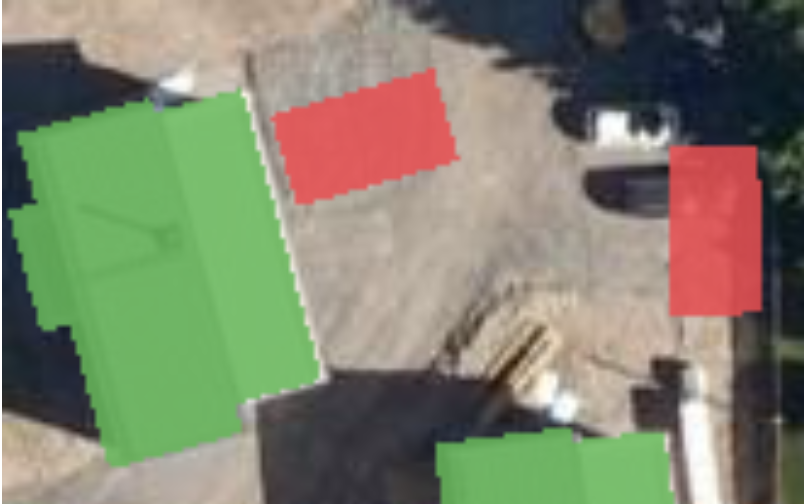
\includegraphics[width=0.5\linewidth]{fig/building_notbuilding}
	\caption{Contradictory information in FKB dataset and aerial image. The red buildings exist in FKB but no not exist in the aerial image \citep{Orstavik2017}}
	\label{fig:buildingnotbuilding}
\end{figure}



